\section{Konzept Datenkommunikation}\label{sec:dKomp}
In diesem Kapitel geht es um die konzeptuelle Ausführung der Datenkommunikation. Es teilt sich auf in die Teile Hardware und Software und ist zugehörig zum Arbeitspaket 5 - Datenkommunikation; genauer AP 5a: Entwicklung eines Hardware- und Software-Konzepts für die Kommunikation und behandelt die Ausführung der notwendigen Daten und deren Kommunikationsmöglichkeiten in Hard- und Software.  Auch die Rechnerarchitektur wird hier beschrieben.\par
Die entsprechenden Hardwarekomponenten sind in Abbildung \ref{fig:dKomp} in violett farblich markiert.
\begin{figure}[hbt]
    \centering
    \pgfdeclarelayer{background}
\pgfdeclarelayer{foreground}
\pgfdeclarelayer{Beschriftung}
%Farbendefinition
\definecolor{elek}{RGB}{105,105,105}%grau{55,126,184}%blau
\definecolor{pneu}{RGB}{105,105,105}%grau{77,175,74}%grün
\definecolor{sens}{RGB}{105,105,105}%grau{228,26,28}%rot
\definecolor{dat}{RGB}{152,78,163}%violett
\definecolor{strom}{RGB}{105,105,105}%grau{0,0,0}%schwarz

\tikzset{wagon/.style={draw = gray, ultra thick, opacity = 0.7}}
\tikzset{seite/.style={opacity = 1}}
\tikzset{elek/.style= {draw = elek, ultra thick, opacity = 1}} %elektrische Komponenten
\tikzset{sens/.style={draw = sens, ultra thick, opacity = 1}} %sensorische Komponenten
\tikzset{pneu/.style={draw = pneu, ultra thick, opacity = 1}} %pneumatische Komponenten
\tikzset{dat/.style={draw = dat, ultra thick, opacity = 1}} %Datenkomponenten
\tikzset{strom/.style={draw = strom, ultra thick, opacity = 1}} %Strom- und Datenleitungen
\tikzset{annotation/.style={draw = black, thick, opacity = 0.7, font=\scriptsize}}

\pgfsetlayers{background,main,Beschriftung,foreground}
\begin{tikzpicture}[scale=0.6]
%%%%%%%%%%%%%%%%%%%%%%%%%%%%%%%%%%%%%%%%%%%%%%%% Hintergrund %%%%%%%%%%%%%%%%%%%%%%%%%%%%%%%%%%%%%%%%%%%%%
    \begin{pgfonlayer}{background}
    %Seiten
        %Seite A
        \path[seite] (0, 3) rectangle +(.6,.2) node[pos = 0.5] (seiteA) {Seite A};
        %Seite B
        \path[seite] (0, -3.2) rectangle +(.6,.2) node[pos = 0.5] (seiteB) {Seite B};
        %Seite 1
        \path[seite] (-12.3, 0) rectangle +(.6,.2) node[pos = 0.5] (seiteB) {Seite 1};
        %Seite 2
        \path[seite] (10.3, 0) rectangle +(.6,.2) node[pos = 0.5] (seiteB) {Seite 2};        
        
    %wagon als Basis
    \path[wagon] (-5,-2) -- (-5,2) -- (5,2) -- (5,-2) -- cycle;
    % HL
    \path[wagon, color=pneu] (-5,-.5) -- (5,-.5) node[pos = 0.6, above] {\color=\gray \tiny{HL}};
    % Buffer
    \begin{scope}[shift = {(-5,1.5)}]
    	\path[wagon] (-.8,.3) -- (0,.3) -- (0,-.3) -- (-.8,-.3);
    	\path[wagon] (-1,.25) -- (-.8,.25) -- (-.8,-.25) -- (-1,-.25);
    	\path[wagon] (-1,-.5) .. controls (-1.05,0) and (-1.05,0) .. (-1,.5);
    \end{scope}
    \begin{scope}[shift = {(-5,-1.5)}]
    	\path[wagon] (-.8,.3) -- (0,.3) -- (0,-.3) -- (-.8,-.3);
    	\path[wagon] (-1,.25) -- (-.8,.25) -- (-.8,-.25) -- (-1,-.25);
    	\path[wagon] (-1,-.5) .. controls (-1.05,0) and (-1.05,0) .. (-1,.5);
    \end{scope}
    \begin{scope}[shift = {(5,-1.5)}, rotate = 180]
    	\path[wagon] (-.8,.3) -- (0,.3) -- (0,-.3) -- (-.8,-.3);
    	\path[wagon] (-1,.25) -- (-.8,.25) -- (-.8,-.25) -- (-1,-.25);
    	\path[wagon] (-1,-.5) .. controls (-1.05,0) and (-1.05,0) .. (-1,.5);
    \end{scope}
    \begin{scope}[shift = {(5,1.5)}, rotate = 180]
    	\path[wagon] (-.8,.3) -- (0,.3) -- (0,-.3) -- (-.8,-.3);
    	\path[wagon] (-1,.25) -- (-.8,.25) -- (-.8,-.25) -- (-1,-.25);
    	\path[wagon] (-1,-.5) .. controls (-1.05,0) and (-1.05,0) .. (-1,.5);
    \end{scope}
    %Wheelset
    \begin{scope}[shift = {(-4,0)}]
    	\path[wagon] (-.1,1.7) -- (.1,1.7) -- (.1,-1.7) -- (-.1, -1.7) -- cycle; 
    	\path[wagon] (-.6,1.4) -- (.6,1.4) -- (.55,1.5) -- (-.55, 1.5) -- cycle; 
    	\path[wagon] (-.6,-1.4) -- (.6,-1.4) -- (.55,-1.5) -- (-.55, -1.5) -- cycle; 
    \end{scope}
        \begin{scope}[shift = {(-2.5,0)}]
    	\path[wagon] (-.1,1.7) -- (.1,1.7) -- (.1,-1.7) -- (-.1, -1.7) -- cycle; 
    	\path[wagon] (-.6,1.4) -- (.6,1.4) -- (.55,1.5) -- (-.55, 1.5) -- cycle; 
    	\path[wagon] (-.6,-1.4) -- (.6,-1.4) -- (.55,-1.5) -- (-.55, -1.5) -- cycle; 
    \end{scope}
    \begin{scope}[shift = {(4,0)}]
    	\path[wagon] (-.1,1.7) -- (.1,1.7) -- (.1,-1.7) -- (-.1, -1.7) -- cycle; 
    	\path[wagon] (-.6,1.4) -- (.6,1.4) -- (.55,1.5) -- (-.55, 1.5) -- cycle; 
    	\path[wagon] (-.6,-1.4) -- (.6,-1.4) -- (.55,-1.5) -- (-.55, -1.5) -- cycle; 
    \end{scope}
    \begin{scope}[shift = {(2.5,0)}]
    	\path[wagon] (-.1,1.7) -- (.1,1.7) -- (.1,-1.7) -- (-.1, -1.7) -- cycle; 
    	\path[wagon] (-.6,1.4) -- (.6,1.4) -- (.55,1.5) -- (-.55, 1.5) -- cycle; 
    	\path[wagon] (-.6,-1.4) -- (.6,-1.4) -- (.55,-1.5) -- (-.55, -1.5) -- cycle; 
    \end{scope}
    \end{pgfonlayer}
%%%%%%%%%%%%%%%%%%%%%%%%%%%%%%%%%%%%%%%%%%%%%%% Vordergrung %%%%%%%%%%%%%%%%%%%%%%%%%%%%%%%%%%%%%%%%%%%%%%%%%
    \begin{pgfonlayer}{foreground} %Komponete
    %elektronische Komponenten
        %Radsatzgenerator
        \path[elek, fill = elek, thin] (-4.3, -1.9) rectangle +(.6,.2) node[pos = 0.5] (wsg) {};
        %Rechner
        \path[elek, fill = elek, thin] (-.5, -1.6) rectangle +(1,.3) node[pos = 0.5] (bcu) {};
        %Batterie
        \path[elek, fill = elek, thin] (-1.8, -1.8) rectangle +(1,.5) node[pos = 0.5] (bat) {};
        %optionale Ladeelektronik
        \path[elek, fill = elek, thin] (-1.8, 1.2) rectangle +(0.8,.4) node[pos = 0.5] (ole) {};
    % pneumatische Komponenten
        %epBremse
        \path[pneu, fill = pneu] (.9,-1.3) rectangle (1.1,-1.5) node[pos = 0.5] (epb) {};
        %Endabsperrhähne
        \path[pneu, fill = pneu] (-5.2, -.4) rectangle (-5,-.6) node[pos = 0.5] (eca) {};
        \path[pneu, fill = pneu] (5.2, -.4) rectangle (5,-.6) node[pos = 0.5] (ecb) {};
        %Aktorik Bremse
        \path[pneu, fill = pneu, thin] (-.5, 0) rectangle +(1,.5) node[pos = 0.5] (bcu2) {};
    %sensorische Komponenten
        %drahtloserSensor
        \path[sens, fill = sens, thin] (3.9, -1.7) rectangle +(.2,-.2) node[pos = 0.5] (wss) {};
        %Flachstellendektektor
        \path[sens, fill=sens, thin] (3.15, 1.8) rectangle +(.2,-.2) node[pos = 0.5] (flachstelle) {};
        \path[sens, fill=sens, thin] (-3.35, 1.8) rectangle +(.2,-.2) node[pos = 0.5] (flachstelle2) {};
        %Laufleistung
        \path[sens, fill = sens, thin] (3.9, 0) rectangle +(.2,-.2) node[pos = 0.5] (ll) {};
    %Datenkomponeten
        %Kurzstreckenfunk
        \path[dat, fill = dat] (-5.2, -.9) rectangle (-5,-1.05)node[pos = 0.5] (sra) {};
        \path[dat, fill = dat] (5.2, -.9) rectangle (5,-1.05)node[pos = 0.5] (srb) {};
        \path[dat, fill = dat] (5.2, .9) rectangle (5,1.05)node[pos = 0.5] (src) {};
        \path[dat, fill = dat] (-5.2, .9) rectangle (-5,1.05) node[pos = 0.5] (srd) {};
    \end{pgfonlayer}
%%%%%%%%%%%%%%%%%%%%%%%%%%%%%%%%%%%%%%%%%%%%%%% Beschriftung %%%%%%%%%%%%%%%%%%%%%%%%%%%%%%%%%%%%%%%%%%%%%%%%%
    \begin{pgfonlayer}{Beschriftung}
    %elektronische Komponenten
        %Radsatzgenerator
        \path[annotation, thin] (wsg) -- +(-.5,-.5) node[left] {Achsdeckelgenerator};
        %Rechner
        \path[annotation, thin] (bcu) -- +(1,-1) node[right] {Bordelektronik};
        %Batterie
        \path[annotation, thin] (bat) -- +(-1,-1) node[left] {Batterie};
        %optionale Ladeelektronik
        \path[annotation, thin] (ole) -- +(-.9,.9) node[left] {externe Ladeschnittstelle};
    %pneumatische Komponenten
        %epBremse
        \path[annotation, thin] (epb) -- +(.4,-.4) node[right] {ep-Bremse};
        %Endabsperrhähne
        \path[annotation, thin] (eca) -- +(-.5,.5) node[left] {Aktor Endabsperrhahn};
        %Aktorik Bremse
        \path[annotation, thin] (bcu2) -- +(.5,.5) node[right] {Aktorik Bremse};
    %sensorische Komponenten
        %drahtloserSensor
        \path[annotation, thin] (wss) -- +(.5,-.5) node[right] {Laufleistung}; 
        %Flachstellen
        \path[annotation, thin] (flachstelle) -- +(.7,.7) node[right] {Lagertemperatur};
        \path[annotation, thin] (flachstelle2) -- +(7.2,.7) node[right] {};
        %Laufleistung
        \path[annotation, thin] (ll) -- +(1.2,.5) node[right] {Beschleunigungen};
    %Datenkomponeten
        %Kurzstreckenfunk
        \path[annotation, thin] (srd) -- +(-.5,-.5) node[left] {Kurzstreckenfunk};    
    \end{pgfonlayer}
%%%%%%%%%%%%%%%%%%%%%%%%%%%%%%%%%%%%%%%%%%%%%% Main %%%%%%%%%%%%%%%%%%%%%%%%%%%%%%%%%%%%%%%%%%%%%%%%%%%%
    \begin{pgfonlayer}{main} %Leitungen
    %elek
        %Radsatzgenerator
        \path[elek] (wsg) +(-.1,0) -| (-3.3, -1);%-- +(1,0) -- (-3.2,-1);
        \path[strom, dashed] (wsg) +(-.1,0) -| (-3.3, -1);%-- +(1,0) -- (-3.2,-1);
        %Rechner
        \path[elek] (bcu) +(0,0)  -- (0,-1);
        \path[strom, dashed] (bcu) +(0,0)  -- (0,-1);
        %Batterie
        \path[elek] (bat) +(0,0)  -- (-1.3,-1);
        \path[strom, dashed] (bat) +(0,0)  -- (-1.3,-1);
        %optionale Ladeelektronik
        \path[elek] (ole) +(0,0)  -- (-1.35,-1);
        \path[strom, dashed] (ole) +(0,0)  -- (-1.35,-1);
    %pneu
        %ep-Bremse
        \path[pneu] (1,-.5) -- (1,-1.3);
        %\path[strom, dashed] (1,-.5) -- (1,-1.3);
        \path[pneu] (epb) +(.1,0) -- +(-.5,0);
        \path[strom, dashed] (epb) +(.1,0) -- +(-.5,0);
        %Endabsperrhähne
        \path[pneu] (eca) +(-.1,0) -- +(.2,0) -- (-4.9,-1);
        \path[strom, dashed] (eca) +(-.1,0) -- +(.2,0) -- (-4.9,-1);
        \path[pneu] (ecb) +(.1,0) -- +(-.2,0) -- (4.9,-1);
        \path[strom, dashed] (ecb) +(.1,0) -- +(-.2,0) -- (4.9,-1);
        %Aktorik Bremse
        \path[pneu] (bcu2) +(0,0)  -- (0,-1);
        \path[strom, dashed] (bcu2) +(0,0)  -- (0,-1);
    %Sensorische Kompoenten
        %Flachstellen
        \path[sens] (flachstelle)+(0,0) -- (3.2, -1);
        \path[strom, dashed] (flachstelle)+(0,0) -- (3.2, -1);
        \path[sens] (flachstelle2) +(0,0)-- (-3.3, -1);
        \path[strom, dashed] (flachstelle2) +(0,0)-- (-3.3, -1);
        %Laufleistung
        \path[sens] (ll)+(0,0) -- (4, -1);
        \path[strom, dashed] (ll)+(0,0) -- (4, -1);
        %drahloser Sensor
        \path[strom, dotted] (wss)+(0,0) -- (4, -1);
    %Strom- und Datenleitung
        \path[dat] (-5,-1) -- (5,-1);
        \path[strom, dashed] (-5,-1) -- (5,-1);
        %Kurzstreckenfunk
        \path[dat] (srd) +(-.1,0) -- +(.3,0) -- (-4.8,-1);
        \path[strom, dashed] (srd) +(-.1,0) -- +(.3,0) -- (-4.8,-1);
        \path[dat] (src) +(.1,0) -- +(-.3,0) -- (4.8,-1);
        \path[strom, dashed] (src) +(.1,0) -- +(-.3,0) -- (4.8,-1);
    \end{pgfonlayer}

\end{tikzpicture}

    \caption{Hardwarekomponenten zur Datenkommunikation des Gesamtsystems}
    \label{fig:dKomp}
\end{figure}
Damit die Wagen untereinander sozial interagieren können, ist eine Kommunikation untereinander ebenso notwendig wie Informationen über sich selbst. Zur Verarbeitung und Sicherung eigener Daten werden Sensoren und Aktoren ausgelesen und im Digitalen Zwilling gespeichert.\par
Dieser Digitale Zwlling wird bei der Kommunikation mit anderen Wagen, der Lok oder mobilen Device je nach Autorisierung mit Lese- oder Lese- und Schreibzugriff ausgetauscht.\par
Der Wagen besitzt, siehe Abbildung \ref{fig:Wagenkomm}, zwei, an den Längsseiten angebrachte, Möglich- keiten für den Kurzstreckenfunk zur Kommunikation mit Nachbarwagen, sowie zwei WLAN-Antennen mit eigener CPU an zwei gegenüberliegenden Ecken als Kommunikationsschnittstelle zum Bediener sowie zur Überbrückung nicht ausgerüsteter Wagen im \gls{Wagenzug}. Zusätzlich hat jeder Wagen zur Ortung und Zeitsynchronisation eine GPS-Antenne und - je nach Ausstattung - eine optionale Möglichkeit für den Fernfunk mittels GSM, GSMR, UMTS oö zum Übersenden von Daten in die Cloud. Die Kommunikation mit Sensoren und Aktoren läuft direkt über den Hauptrechner. Dieser ist leistungsstärker und beinhaltet neben der Verarbeitung der Sensor- und Aktordaten auch das Batteriemanagementsystem, sowie die Digitale Identität.\par
\begin{figure}[hbt]
    \centering
    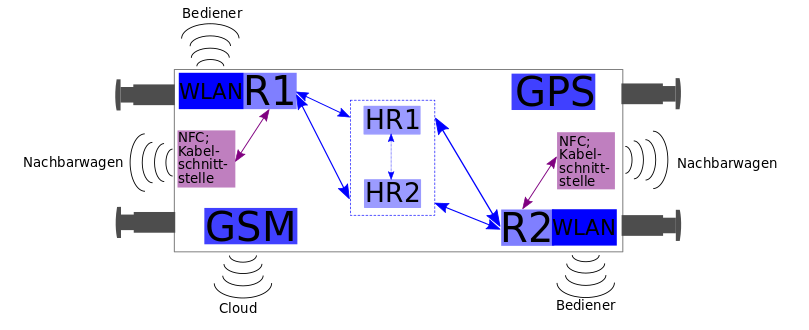
\includegraphics[width=\textwidth]{Bilder/wagen_draufsicht.png}
    \caption{Kommunikationsmöglichkeiten und angedeutete Rechnerstruktur eines einzelnen Güterwagen 4.0}
    \label{fig:Wagenkomm}
\end{figure}
Die Kommunikation im Wagen findet über ein Bussystem mit geringem spezifischen Energiebedarf statt. Für erste Tests ist EtherCAT angedacht.\par
Die Kommunikation der Wagen untereinander findet entweder, bei nicht vollständig ausgerüsteten Wagenzügen, über ein WLAN-Mesh (siehe Abbildung \ref{fig:Wagenkomm}, blau) in mittlerer Distanz oder direkt über eine Kurzdistanz-Verbindung (lila) statt. Diese Kurzdistanzverbindungen können kabelgebunden über Ethernet, NFC, WLAN mit 60GHz oder BlueTooth entstehen. Eine sinnvolle Auswahl wird im Projekt getroffen. Bei beiden Kommunikationswegen ist wichtig, dass diese sicher und unempfindlich gegenüber Störungen und Manipulation ist. Sie soll außerdem über Kurz- und Mittelstreckenfunk redundant ausgeführt sein, was zu einer  höheren Sicherheit und Zuverlässigkeit führt. Siehe dazu auch Abbildung \ref{fig:Zugkomm}. \par
Zusätzlich soll auch noch eine optionale Verbindung zu einer Cloud im Fernbereichsfunk zur Verfügung stehen. Diese erhält allerdings nur einen Lesezugriff um eine Manipulation über die Cloud so schwierig wie möglich zu gestalten.\par
\begin{figure}[hbt]
    \centering
    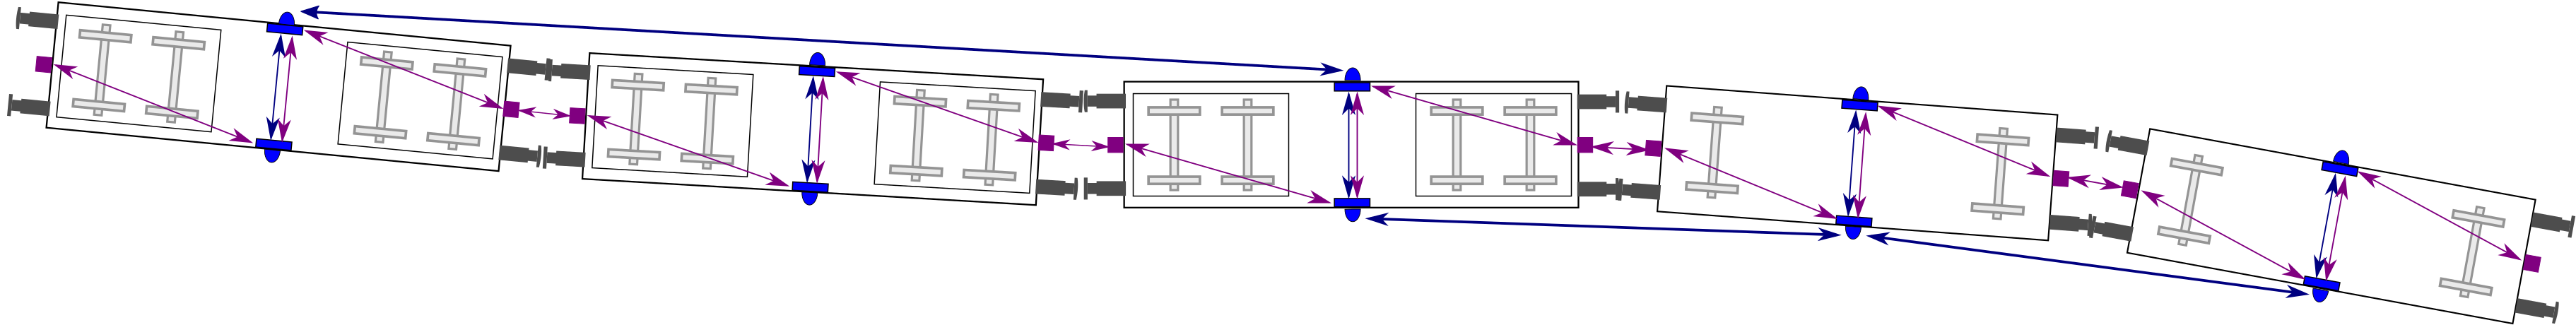
\includegraphics[width=\textwidth]{Bilder/zug_draufsicht_bogen.png}
    %\includesvg[width=\textwidth]{Bilder/zug_draufsicht_bogen}
    \caption{Kommunikation im Zugverband\cite{autonBetrieb}}
    \label{fig:Zugkomm}
\end{figure}
Die Kommunikation mit dem Bediener erfolgt lokal innerhalb des wageneigenen WLANs, bzw. des \gls{Wagenzug}es eigenen WLAN-Meshs. Eine genaue Ausarbeitung dieser Kommunikation erfolgt im Projekt. Möglich wären beipielsweise einzelne Bedienelemente mittels RFID oder QR-Code anzuwählen und am mobilen Endgerät zu bedienen.\par
Bei einer Vollausrüstung von Wagen mit Kommunikation von Wagen zu Wagen über Funk und innerhalb der Wagen über EtherCAT ist diese Kommunikation kaum störbar. Hier bietet der \gls{Gueterwagen} auch volles Potential für Zugautomatisierungen inklusive Zugtaufe, \gls{Bremsprobe} und \gls{ep-Bremsen}n. Sogar ETCS Level 3 kann möglich sein.\par
Aber auch bei nur einer Teilausrüstung der Wagen kann eine Nutzentfaltung durch Digitalisierung von Prozessen an der Ladestelle stattfinden. Eine Automatisierung ist dann in Verbindung mit stationärer Technik im Betrieb möglich.\par
Die Vernetzung zur Lok kann mittels eines Dongles an der UIC 556-Schnittstelle über das Wire-Train-Bus-Gateway stattfinden. Dies ist als Idee angedacht, wird aber nicht im Projekt umgesetzt.\par

\paragraph{Rechnerstruktur}
Damit eine sichere Datenhaltung und -übertragung möglich ist, wird die in Abbildung \ref{fig:Wagenkomm} gezeigte Rechnerarchitektur für den Hauptrechner vorgeschlagen. Diese ist eine Überlegung, muss aber noch nicht für das Labormuster oder den Demonstrator aufgebaut werden.\par
Der in der Mitte gezeigte Hauptrechner besteht aus zwei getrennten Kernen. Diese sorgen für eine Zweikanaligkeit im sicherheitskritischen Bereich. Ebenfalls zweikanalig ausgeführt ist, wie oben beschrieben, die Kommunikation mit den anderen Wagen.\par
Angedeutet sind der Bediener, dessen Schnittstelle der Nahbereichsfunk darstellt, das GSM-Modul, die Schnittstelle zur Cloud und die Sensoren, Aktoren und Kommunikationseinheiten im Wagen.\par
Die beiden Kerne im Hauptrechner tauschen sich gegenseitig rückkopplungsfrei aus und geben ihre Befehle zweikanalig an Sensoren, Aktoren und die Kommunikationseinheiten im Wagen weiter. Die zurückkommenden Informationen (rote Pfeile zu Rechner 1 und Rechner 2) werden von den Rechnern verarbeitet und im Speicher gesichert.\par
Befehle aus der Nahbereichsschnittstelle werden vom Bediener gegeben und nach Autorisierung verarbeitet. \par

\paragraph{Softwarestruktur}
Die Softwarestruktur, siehe das Diagramm in Abbildung \ref{fig:SWStruktur}, zeigt den Hauptrechner HR sowie die beiden Kommunikationsmodule R1 und R2 im \gls{Gueterwagen 40}. Angenzend dazu sind andere Wagen und ein Bediener angedeutet.
Alle Rechner sind mit einem Linuxsystem auszustatten. Zu erkennen ist, dass die beiden Kommunikationsrechner nur Schnittstellen zum Hauptrechner und zur Kommunikation mit weiteren Wagen sowie zum Bediener haben. Der Hauptrechner dagegen ist leistungsstärker und verarbeitet alle hereinkommenden Daten. Dazu gehört das BMS, die Digitale Identität, alle Sensor- und Aktordaten. Ebenso wird hier die Zugzusammenstellung und Zugtaufe ebenso wie der virtuelle Bremszettel verarbeitet. Er bietet die Intelligenz des Güterwagens 4.0.\par
Die Software selbst soll vorallem intern arbeiten und über generische Netzwerkschnittstellen kommunizieren. So kann ein häufiges verändern der Software durch Änderungen in der Hardware vermieden werden. Die Kommunikation mit der Hardware kann dann beispielsweise über eine REST-Schnittstelle erfolgen.

\begin{figure}
    \centering
    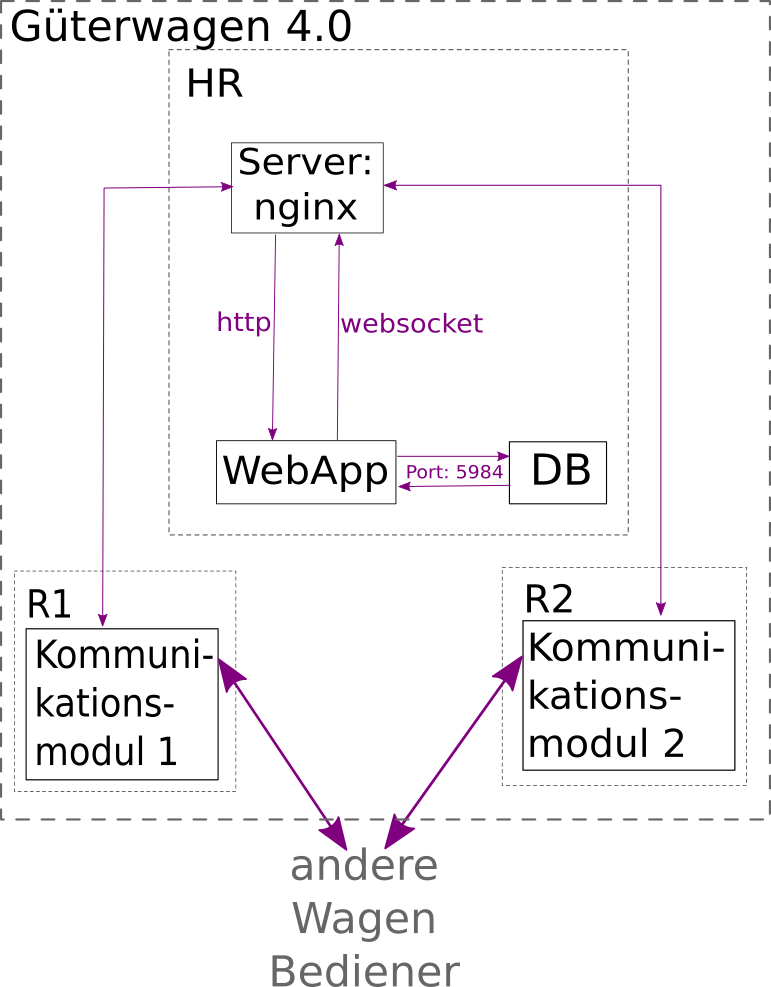
\includegraphics[width=10cm%\textwidth
    ]{Bilder/Softwarestruktur.png}
    \caption{Softwarestrukturdiagramm des Güterwagen 4.0}
    \label{fig:SWStruktur}
\end{figure}


\begin{comment}
\subsubsection{Hardware}
An Hardwarekomponenten sind Funkstellen für die Wagenkommunikation geplant.
\begin{itemize}
    \item Komponenten für Kurzstreckenfunk -- WLAN 60GHz/2,4GHz -- Wagen-Wagen, Wagen-Lok -- 1b
    \item Komponenten für mittlere Distanzen -- Wagen...Wagen, Wagen-Device
    \item Komponenten für Fernbereichsfunk -- Wagen-Cloud
\end{itemize}
\subsubsection{Software}
\begin{itemize}
    \item Lademanagement \label{sec:Lademanagment} -- 3d
    \item Anforderungen an sicheres funkgestütztes Bedienen und beobachten bei der Zugbildung -- 1d
    \item DI -- 1c
    \item \gls{WagonOS}
    \item Kommunikationsprotokolle - Datenkommunikation -- 1c
    \item automatische Zugbildung -- 1c
    \item automatische Bremsprobe -- 1c
    \item automatische Bremseinstellung
\end{itemize}
\end{comment}
